\documentclass[12pt]{article}
\usepackage[utf8]{inputenc}
\usepackage[french]{babel}
\usepackage{amsmath,amsthm,amsfonts,amssymb}
\usepackage{lmodern}
\usepackage[top=2.4cm,bottom=2.4cm,left=2cm,right=2cm]{geometry}
\usepackage{hyperref}
\usepackage{multicol}
\usepackage{enumitem}
\usepackage{listings}
\usepackage[dvipsnames]{xcolor}
\usepackage{tikz}

%\date{}
\title{{\bf  Génie logiciel} \\
	Notes du cours de 09/12  \\
	{\small L3 Informatique appliquée 2022-2023} \\
	{\it \small MABROUK Fayez}}
\begin{document}
	\maketitle
	\newpage
	\section{Conception de logiciels}
	\subsection{Définitions}
	\begin{itemize}
		\item[* ] Définition : La conception logicielle est le processus de définition de la structure globale et de 
		interaction de votre code afin que le produit résultant satisfasse aux exigences.
		\item[* ] La modélisation est différente de la conception !.
		\item[* ] La modélisation : un moyen d'exprimer la conception.
		\item[* ] C'est une étape importante pour se mettre d'accord.
		\begin{itemize}
			\item[* ] sur l'utilisation du produit logiciel.
			\item[* ] sur la structure du produit logiciel.
		\end{itemize}
	\end{itemize}
\subsection{Concepts de conception de logiciels}
\begin{itemize}
	\item[* ] L'abstraction.
	\item[* ] Couplage et cohésion.
	\item[* ] Décomposition et modularisation.
	\item[* ] Encapsulation et masquage de l'information.
	\item[* ] Séparation de l'interface et de l'implémentation.
	\item[* ] Suffisance, complétude et primitivisme.
	\item[* ] Séparation des préoccupations.
\end{itemize}
\subsection{Abstraction}
\begin{itemize}
	\item[* ] \textbf{Abstraction} : une vue d'un objet qui se concentre sur l'information pertinente pour un objectif particulier et ignore le reste de l'information.
	\item[* ] Sans abstraction, votre programme devient trop complexe et inutilisable.
	\item[* ] Vous devez toujours vous poser la question suivante : "Quelle est la complexité adaptée à mon objectif ?"
	
\end{itemize}
\subsection{Encapsulation}
\begin{itemize}
	\item[* ] \textbf{Encapsulation} : cacher les détails d'une abstraction à une entité externe.
	\item[* ] Composant essentiel d'une abstraction, mais différent de l'abstraction.
\end{itemize}
\subsection{Modularisation}
\begin{itemize}
	\item[* ] Modularisation : diviser le logiciel en petits composants, chacun ayant une
	interface bien définie.
	\item[* ] Principe "diviser pour régner".
	\item[* ] Réalisé grâce à l'encapsulation : ce qui n'est pas pertinent pour l'utilisateur externe est
	caché.
	\item[* ] Advantages:
	\begin{itemize}
		\item[* ] Plus facile à maintenir.
		\item[* ] Plus facile de travailler en parallèle.
		\item[* ] Gère bien la complexité.
	\end{itemize}
\end{itemize}
\subsection{Séparation des préoccupations}
\begin{itemize}
	\item[* ] La séparation des préoccupations est un principe de conception qui stipule qu'un programme doit être divisé en sections, chacune répondant à une préoccupation différente.
	\item[* ] Terme inventé par Dijkstra en 1974.
	\item[* ] Chaque section est un module.
	\item[* ] Permet la réutilisation des modules.
\end{itemize}
\subsection{Séparation de l'interface et de l'implémentation}
\begin{itemize}
	\item[* ] Séparation de l'interface et de l'implémentation : l'interface est publique, mais pas l'implémentation.
	détails de l'implémentation.
	\item[* ] L'interface décrit les services qu'un client de la classe peut utiliser, et comment les
	les demander.
	\item[* ] L'implémentation décrit comment ces services sont fournis.
\end{itemize}
\subsection{Couplage et cohésion}
\begin{itemize}
	\item[* ] Le couplage est la mesure du degré d'interdépendance entre les modules
	du logiciel.
	\item[* ] En général, il faut viser un faible couplage.
\item[* ] La cohésion est la mesure du degré de relation fonctionnelle entre les éléments du module
du logiciel sont fonctionnellement liés.
\item[* ] En général, il faut viser une cohésion élevée.
\end{itemize}
\subsection{Suffisance, exhaustivité et primitivité}
\begin{itemize}
	\item[* ] Un composant logiciel doit être :
	\begin{itemize}
		\item[* ] suffisant et complet : il capture toutes les caractéristiques importantes d'une abstraction
		et rien de plus.
		\item[* ] Primitif : la conception doit être basée sur des modèles faciles à mettre en œuvre.
	\end{itemize}
\end{itemize}
\subsection{Patrons de conception : pourquoi ?}
\begin{itemize}
	\item[* ] La plupart des problèmes de conception de logiciels sont communs à de nombreux projets
	\item[* ] Pas besoin de réinventer la roue
	\item[* ] Permettre des solutions communes
\end{itemize}
\subsection{Modèles de conception : quoi ?}
\begin{itemize}
	\item[* ] Définition : " solution générale, réutilisable, à un problème qui se pose couramment
	dans un contexte donné de conception de logiciels ".
	\item[* ] Concept proposé par Christopher Alexander en 1977
	\item[* ] Formalisé (et popularisé) par le " Gang of Four " en : 
		\begin{figure}[!hbtp]
		\centering
		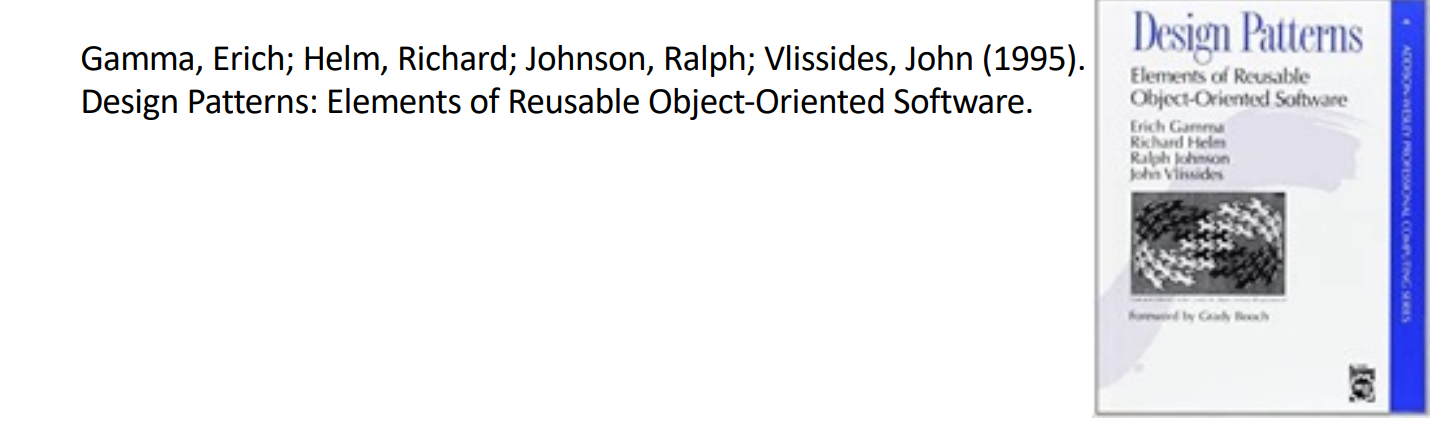
\includegraphics[scale=0.75]{Capture.PNG}
		%\caption{Légende de l'image}
	\end{figure}
\item[* ] 23 modèles de conception répartis en 3 catégories :
\begin{itemize}
	\item[* ] Creational : patterns permettant de créer un objet
	\item[* ] Structurel : patterns qui composent des classes pour obtenir de nouvelles fonctionnalités
	\item[* ] Behavorial : patterns qui traitent de la communication entre objets.
\end{itemize}
\end{itemize}
\subsection{Modèles de conception créatifs - Singleton}
\begin{itemize}
	\item[* ] Garantit qu'une classe n'a qu'une seule instance.
	\item[* ] Meilleure alternative aux variables globales.
	\item[* ] Exemple de cas d'utilisation : logger
	\begin{figure}[!hbtp]
		\centering
		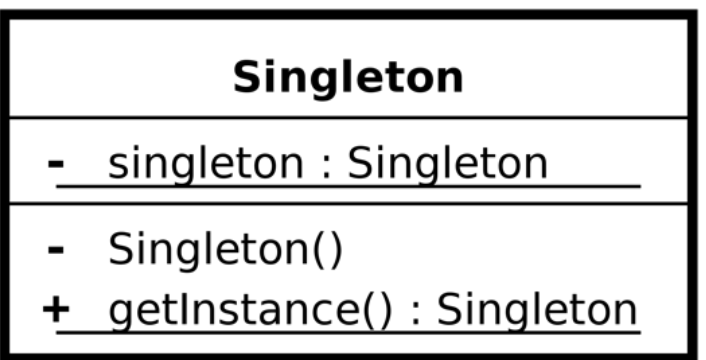
\includegraphics[scale=0.75]{Capture1.PNG}
		%\caption{Légende de l'image}
	\end{figure}
\end{itemize}
\subsection{Modèles de conception structurels - Décorateur}
\begin{itemize}
	\item[* ] Ajoute un comportement à un objet individuel
	individuel de manière dynamique.
	\item[* ] Peut être considéré comme une
	spécialisation
	\item[* ] Souvent utilisé pour les interfaces graphiques.
	\newpage
	\begin{figure}[!hbtp]
		\centering
		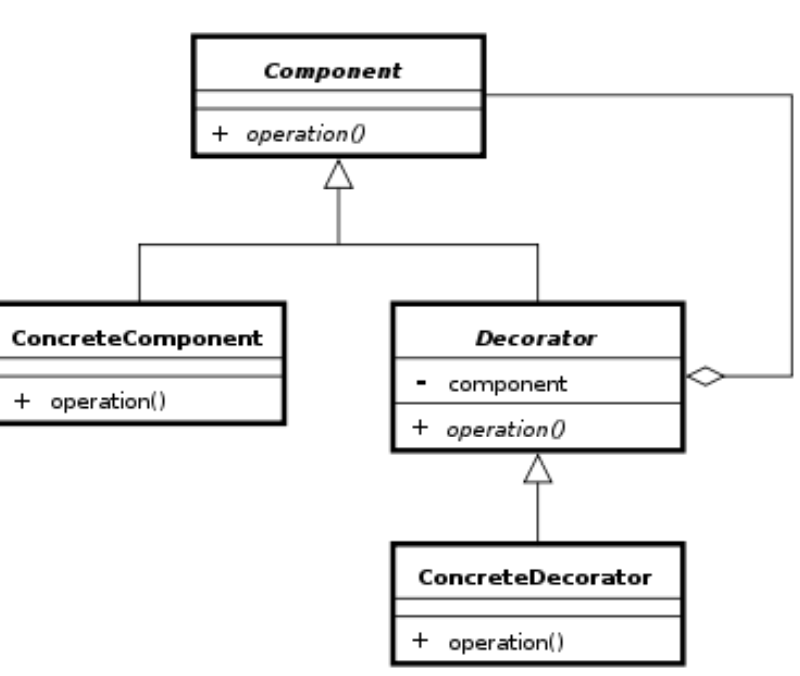
\includegraphics[scale=0.75]{Capture2.PNG}
		%\caption{Légende de l'image}
	\end{figure}

\end{itemize}
\begin{figure}[!hbtp]
	\centering
	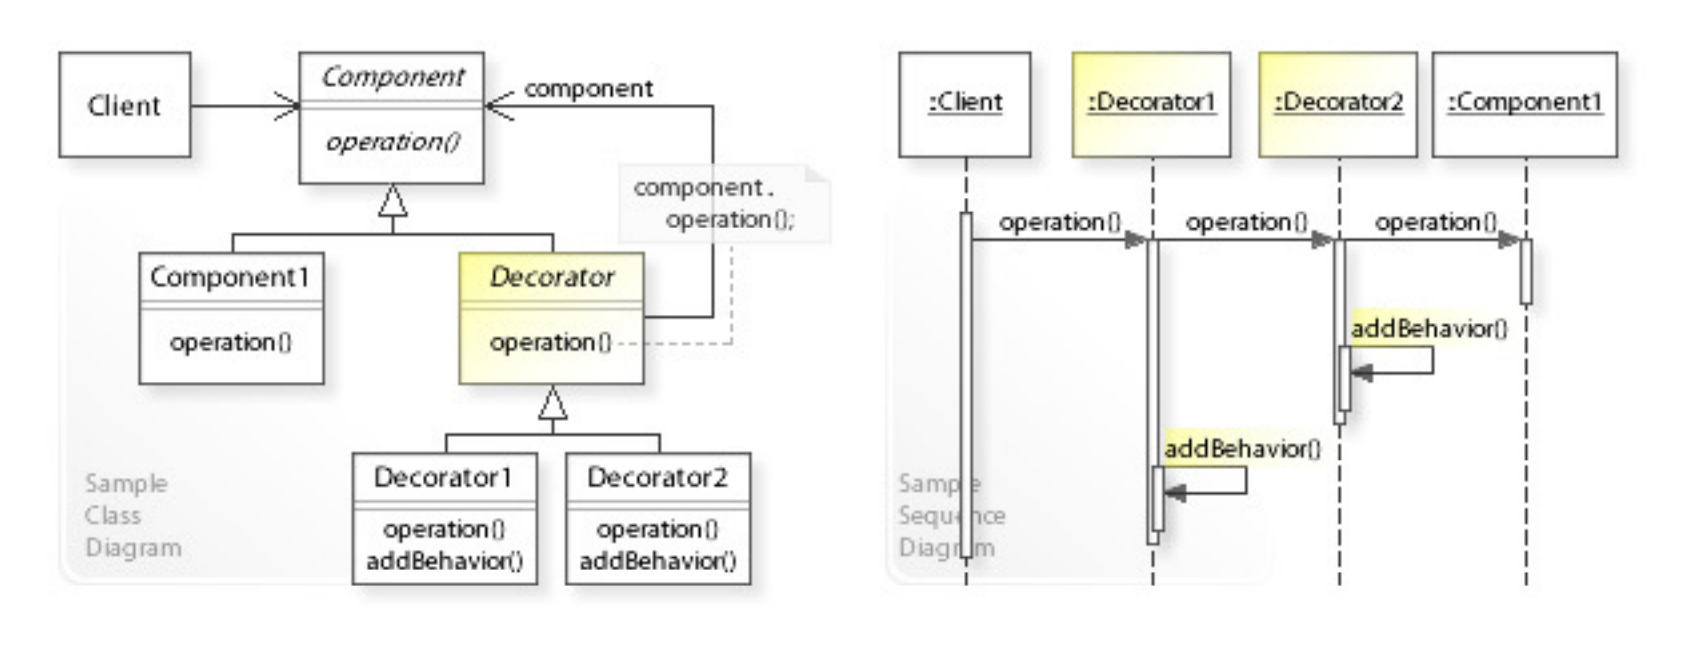
\includegraphics[scale=0.75]{Capture3.PNG}
	%\caption{Légende de l'image}
\end{figure}
\subsection{Modèles de conception comportementale - Observer}
\begin{itemize}
	\item[* ] Permet les dépendances sans
	couplage
	\item[* ] Exemple de cas d'utilisation : s'abonner
	pour la disponibilité d'un produit.
	\begin{figure}[!hbtp]
		\centering
		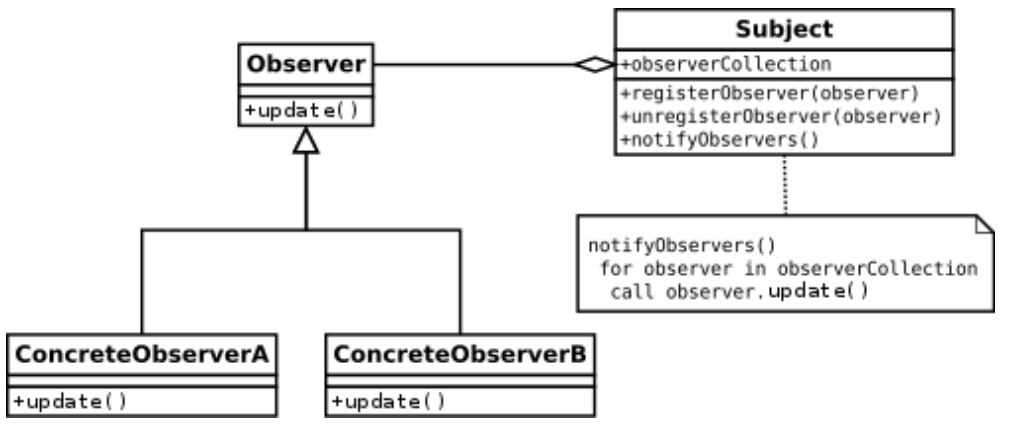
\includegraphics[scale=0.75]{Capture4.PNG}
		%\caption{Légende de l'image}
	\end{figure}
\end{itemize}
\subsection{Critiques sur les modèles de conception}
\begin{itemize}
	\item[* ] Le langage de programmation de haut niveau apporte souvent des solutions à ces problèmes.
	\item[* ] Souvent, les gens essaient de trop les appliquer. Les design patterns ne sont pas les
	solutions à tous les problèmes.
	\item[* ] Une solution spécifique pourrait mieux convenir à votre projet.
	\item[* ] Utilisez-les avec parcimonie
\end{itemize}
\subsection{Conclusion}
\begin{itemize}
	\item[* ] La conception de logiciels est une étape critique vers la création de logiciels de qualité.
	\item[* ] Elle permet de s'assurer que les exigences seront satisfaites.
	\item[* ] Permet une mise en œuvre plus facile.
	\item[* ] Vous devez :
	\begin{itemize}
		\item[* ] Viser à remplir les concepts classiques de conception
		\item[* ] Viser un modèle sur lequel tout le monde est d'accord.
		\item[* ] opter pour les solutions les plus simples possibles
	\end{itemize}
\end{itemize}
\end{document}